\documentclass[12pt, oneside]{article}
\usepackage[letterpaper, margin=1in, headsep=0.5in, left=0.3in, right=2.5in]{geometry}
\usepackage[english]{babel}
\usepackage[utf8]{inputenc}
\usepackage{amsmath}
\usepackage{amsfonts}
\usepackage{amssymb}
\usepackage{tikz}
\usepackage{yhmath}
\usetikzlibrary{quotes, angles}
\usepackage{graphicx}
\usepackage{enumitem}
\usepackage{multicol}

\newif\ifmeta
\metatrue %print standards and topics tags

\title{Regents Geometry}
\author{Chris Huson}
\date{May 2022}

\usepackage{fancyhdr}
\pagestyle{fancy}
\fancyhf{}
\renewcommand{\headrulewidth}{0pt} % disable the underline of the header
\raggedbottom

%\fancyhead[LE]{\thepage}
\fancyhead[RO]{Name:}
\fancyhead[LO]{BECA / Dr. Huson / Geometry Regents Mixed Review}
\cfoot{\thepage}

\begin{document}
\subsubsection*{11.13 Similarity algebra}
\begin{enumerate}[itemsep=1.2cm]
  \item In the diagram below $\triangle ABC \sim \triangle DEF$, $DE=9$, $AB=x$, $AC=2x$, $DF=4x-6$. \\[0.25cm] 
  Determine the length of $\overline{AB}$.
    \begin{center}
      \begin{tikzpicture}[scale=1]
      \coordinate [label=above left:$A$](A) at (85:2);
      \coordinate [label=below:$B$](B) at (0, 0);
      \coordinate [label=right:$C$](C) at (-20:3);
        \draw [thick] (A)--(B)--(C)--cycle;
        \node at (95:1)[left]{$x$};
        \node at (35:1.75)[right]{$2x$};
        \draw [thick, xshift=5cm, yshift=0.5cm] (85:3) node[above]{$D$}--
        (0,0) node[below]{$E$}--
        (-20:4.5) node[right]{$F$}--cycle;
        \draw [thick, xshift=5cm, yshift=0.5cm](90:1.5) node[left]{$9$};
        \draw [thick, xshift=5cm, yshift=0.5cm](30:2.75) node[right]{$4x-6$};
    \end{tikzpicture}
    \end{center}

\item Write an equation of the line that is parallel to the line whose equation is $2x-3y=4$ and passes through the point $(1,7)$.
  
\item Find the volume of a cone with a base circumference of 12 inches and height of 7 in., to the \emph{nearest cubic inch}.

\item What are the coordinates of the center and the length of the radius of the circle whose equation is $x^2+(y-5)^2=36$?

\item In right triangle $ABC$, hypotenuse $\overline{AB}$ has a length of 17.5 cm, and side $\overline{BC}$ has a length of 7.1 cm. What is the measure of angle $B$, to the \emph{nearest degree}?

\item The endpoints of directed line segment $PR$ have coordinates of
$P(0,-2)$ and $R(4,10)$. What are the coordinates of point $Q$, on $\overline{PR}$, that divide $\overline{PR}$ into a ratio of 3:1?

\item For the acute angles in a right triangle, $\sin (70^\circ) =\cos (2x -10)^\circ$. \\
What is the number of degrees in the measure of the smaller angle?

\item In right triangle $RST$ below, altitude $\overline{SV}$ is drawn to hypotenuse $\overline{RT}$.
  \begin{center}
    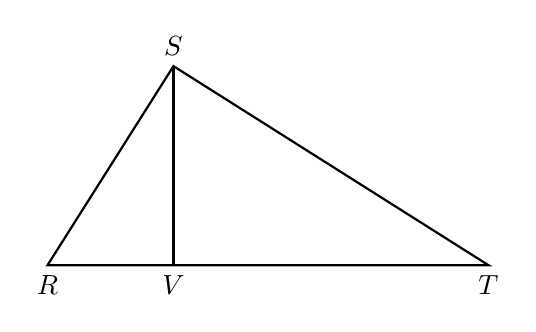
\begin{tikzpicture}[scale=0.8]
    \draw [thick]
    (0,0)node[below]{$R$}--
    (7,0)node[below]{$T$}--
    (2,3.16)node[above]{$S$}--cycle;
    \draw [thick](2,0)node[below]{$V$}--(2,3.16);
  \end{tikzpicture}
  \end{center}
If $RV=2.5$ and $TV=8.1$, what is the length of $\overline{ST}$, to the \emph{nearest tenth}?

\item The secants $\overline{ABC}$ and $\overline{ADE}$ intersect the circle $O$, as shown in the diagram. \\Given $m \wideparen{BD}=44^\circ$ and $m \wideparen{CE}=140^\circ$.
  \begin{enumerate}
    \item Find the $m\angle CDE$, $m\angle CBE$.
    \item Find the $m\angle C$, $m\angle E$.
    \item Find the $m\angle A$.
    \item Two similar triangles are shown. Write a similarity statement, listing the triangles' vertices in corresponding order.
  \end{enumerate}
  \begin{center}
  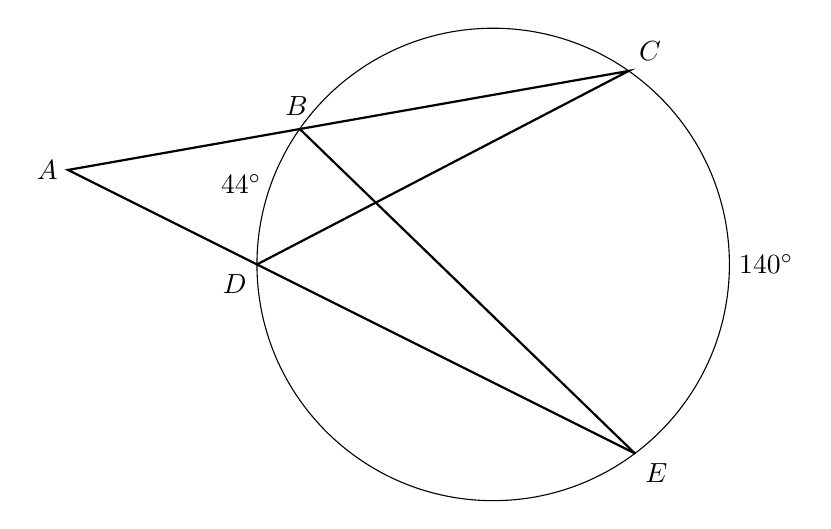
\begin{tikzpicture}[scale=.6]
    \draw (0,0) circle[radius=5];
    \draw [thick]
    (3,-4) node[below right] {$E$}--
    (-5,0) node[below left] {$D$}--
    (-9,2) node[left] {$A$}--
    (55:5) node[above right] {$C$}--
    (-5,0);
    \draw [thick] (3,-4)--(145:5);
    \draw (138:5) node[left] {$B$};
    \draw (0:5) node[right] {$140^\circ$};
    \draw (160:5) node[left] {$44^\circ$};
  \end{tikzpicture}
  \end{center}
  
\end{enumerate}
\end{document}
  